%\part{Konstruktion}
%\chapter{Programmlogik}

\section{QueryCreation}

\begin{figure}[htb]
   \centering
  	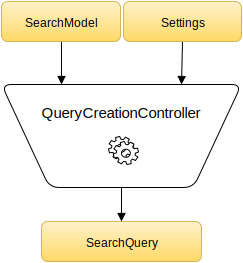
\includegraphics[width=0.4\textwidth]{QueryCreation}
  	\caption{Aufbau des Moduls \lstinline|QueryCreation|}
\end{figure}
\lstinline|QueryCreation| generiert aus den Suchwörtern (\lstinline|SearchModel|) und den Geräte- und App-Einstellungen ein allgemeines Anfrageformat. Dieses Anfrageformat wird in \lstinline|QueryResolution| zu einem für jede Suchmaschine spezifischen Suchformat umgewandelt.

\subsection{QueryCreationCtrl}

%\subsubsection{Unterteilabschnitt}
%\paragraph{Paragraph}
%\subparagraph{Unterparagraph}
